\tikzset{
    table/.style={
           rectangle,
           draw=black, very thick,
           rounded corners,
           text centered,
           },
}

\begin{figure*}[!ht]
\centering
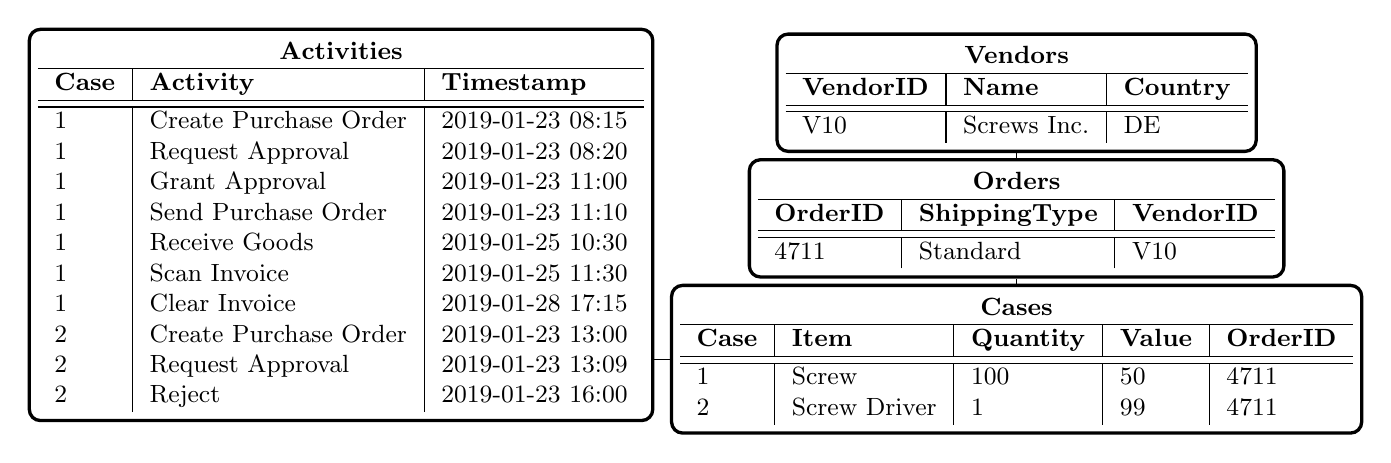
\begin{tikzpicture}
\begin{small}

       \node[table] (ACTIVITIES) 
       {
                \begin{tabular}{l|l|l}
                 \multicolumn{3}{c}{\textbf{\textsc{Activities}}} \\ \hline
                 \textbf{\textsc{Case}} & \textbf{\textsc{Activity}} & \textbf{\textsc{Timestamp}}  \\
                       \hline
                       \hline
                       1 & Create Purchase Order & 2019-01-23 08:15\\
                       1 & Request Approval & 2019-01-23 08:20\\
                       1 & Grant Approval & 2019-01-23 11:00\\
					   1 & Send Purchase Order & 2019-01-23 11:10\\
					   1 & Receive Goods & 2019-01-25 10:30\\
					   1 & Scan Invoice & 2019-01-25 11:30\\
					   1 & Clear Invoice & 2019-01-28 17:15\\
					   2 & Create Purchase Order & 2019-01-23 13:00\\
                       2 & Request Approval & 2019-01-23 13:09\\
                       2 & Reject & 2019-01-23 16:00\\
               \end{tabular}
       };
 
 
       \node[table] (CASES) at ([xshift=4.6cm,yshift=0.8cm]ACTIVITIES.south east)
       {
               \begin{tabular}{l|l|l|l|l}
                       \multicolumn{5}{c}{\textbf{\textsc{Cases}}} \\
                       \hline
                       \textbf{\textsc{Case}} & \textbf{\textsc{Item}} & \textbf{\textsc{Quantity}} & \textbf{\textsc{Value}} & \textbf{\textsc{OrderID}} \\
                       \hline
                       \hline
                       1 & Screw & 100 & 50 & 4711 \\
                       2 & Screw Driver & 1 & 99 & 4711 \\
               \end{tabular}
       };
      

       \node[table] (ORDERS) at ([yshift=0.83cm]CASES.north)
       {
               \begin{tabular}{l|l|l}
                       \multicolumn{3}{c}{\textbf{\textsc{Orders}}} \\
                       \hline
                       \textbf{\textsc{OrderID}} & \textbf{\textsc{ShippingType}} & \textbf{\textsc{VendorID}} \\
                       \hline
                       \hline
                       4711 & Standard & V10 \\
               \end{tabular}
       };
            
            
       \node[table] (VENDORS) at ([yshift=0.83cm]ORDERS.north)
       {
               \begin{tabular}{l|l|l}
                       \multicolumn{3}{c}{\textbf{\textsc{Vendors}}} \\
                       \hline
                       \textbf{\textsc{VendorID}} & \textbf{\textsc{Name}} & \textbf{\textsc{Country}} \\
                       \hline
                       \hline
                       V10 & Screws Inc. & DE \\
               \end{tabular}
       };
            
      
      
       
       \draw ([yshift=0.8cm]ACTIVITIES.south east) -- (CASES.west) ;
       %\node at ([yshift=1.125cm,xshift=0.2cm]ACTIVITIES.south east) {N} ;
       %\node at ([yshift=0.2cm,xshift=-0.2cm]CASES.west) {1} ;
       \draw (CASES.north) -- (ORDERS.south) ;
       %\node at ([yshift=0.2cm,xshift=-0.2cm]CASES.north) {N} ;
       %\node at ([yshift=-0.2cm,xshift=-0.2cm]ORDERS.south) {1} ;
       \draw (ORDERS.north) -- (VENDORS.south) ;
       %\node at ([yshift=-0.2cm,xshift=-0.2cm]VENDORS.south) {1} ;
       %\node at ([yshift=0.2cm,xshift=-0.2cm]ORDERS.north) {N} ;
       
\end{small}


\end{tikzpicture}
       \caption{Example data model with four tables, including activity and case tables}
       \label{fig:data-model-example}
\end{figure*}
\setlength{\textfloatsep}{0cm}

\section{Introdution}
\label{sec:introduction} 

Enterprises collect large volumes of logged process data from enterprise application software
such as ERP (Enterprise Resource Planning), CRM (Customer Relationship Management),
or SCM (Supply Chain Management) systems. Process data is among the most
valuable assets of a company as it can provide answers to critical business
questions like ``What do the processes in our company look like?", ``Where are
our processes inefficientt?'', or ``How can our processes be improved?''. Process
mining~\cite{process-mining} analyzes process data to answer these questions.
This allows enterprises to get a fact-based view on the performance of their
business, to pinpoin inefficiencies, and to counteract on them.

A key success factor for any process mining tool is a suitable query
language for translating business questions into executable queries over process data. 
%that efficiently analyze and consolidate the process data. 
Although process data is a good fit for the relational model, SQL unfortunately is not well suited for process mining for the following reasons:

\begin{itemize}
\item \textbf{Usability}: Expressing process mining business questions in SQL is tricky and cumbersome
\item \textbf{Performance}: State-of-the-art query optimizers generate poor plans for these complex SQL queries
\end{itemize}

At Celonis, we decided to depart from SQL and develop a new solution tailored
towards the needs of process mining. In particular, we designed \emph{Celonis PQL}, a novel query language for process mining, and we developed \emph{Saola}, a highly efficient database system to process Celonis PQL. 

Celonis PQL is the basis for a commercial product that delivers business
intelligence by interactive process mining. Saola must therefore meet high 
standards in terms of runtime performance, scalability, and latency. 
Saola is highly optimized for drill downs~\cite{drill-down} that
analyze large data sets with hundreds of millions of events in an interactive
fashion. Interactive speed is critical as slow response times
may interrupt a users' train of thought and adversely affect the user
experience. Thus, SaolaDB was designed to process Celonis PQL efficiently.

Besides performance, customers request a system that is easy to setup and maintain. They are reluctant to add yet another database into their IT landscape that must be administrated at high costs. Therefore, Saola was also designed to be usable out-of-the-box without requiring workload-specific fine-tuning by a database administrator.

\par\smallskip\noindent \textbf{Outline.} The remainder of the paper is
structured as follows: Section~\ref{sec:preliminaries} provides background
information on process mining. Section~\ref{sec:celonis-pql} introduces Celonis
PQL, our novel process mining query language, and highlights the main
differences to SQL. Section~\ref{sec:pql-query-engine} introduces our query
engine, Saola, which we evaluate in Section~\ref{sec:evaluation}. We finally
concIude in Section~\ref{sec:conclusion}.
